\section{Experimental Evaluation}\label{sec:exp}
We evaluate our techniques on two real-world trajectory datasets: \pt{} and \sz{}.
\pt{}~\cite{pt} contains a total of 2.39 million taxi trajectories and 75.67 million of GPS points, and the longest trajectory has 3,490 GPS points.
\sz{}~\cite{sz} consists of 3.07 million taxi trajectories with 53.53 million GPS points, and the longest trajectory has 2,268 GPS points. All experiments are conducted on a machine with an Intel i7-8700 CPU, 24 GB memory and an NVIDIA GeForce GTX1080 GPU with 8 GB on-chip memory, running on Windows 10. All methods are implemented in Java 1.8, and the Processing 3 library~\cite{p3} is used for rendering. All datasets and source codes required to reproduce our results are available at~\cite{code}.

This section is organized as follows. In Section~\ref{sec:case}, we present a case study of the visualization results on the \pt{} dataset to demonstrate the merits of our methods. In Section~\ref{sec:user}, we conduct a comprehensive user study to test the effectiveness of our visualization results on practical  tasks including \textit{region center identification}, \textit{reachable route inspection} and \textit{traffic flow comparison}. In Section~\ref{sec:quality}, we quantitatively evaluate the fidelity loss and efficiency of our methods.
%For the sake of page limitation, we briefly present the case of \pt{} in section~\ref{sec:case}, and refer the interested reader to our technical report \cite{techreport} for more cases of \pt{} and \sz{}.
%We then conduct a user study to demonstrate the superiority of our proposal in three real-world applications in Section~\ref{sec:user}.
%to demonstrate the effectiveness and efficiency of our proposal.
% and has been cleaned for further analysis.
% In Section~\ref{sec:case}, we evaluate the effectiveness of our proposal by the case studies on \pt{} and \sz{} trajectory dataset, respectively.
% We then conduct a user study to demonstrate the superiority of our proposal in three real world applications in Section~\ref{sec:user}.
% Last, we perform a qualitative evaluation in Section~\ref{sec:quality} at last.
% We conducted all experiments on a machine with Intel i7-8700, 3.2 GHertz CPU, 24 GBytes memory and NVIDIA GeForce GTX1080, 8 GHertz VRAM GPU, running on Windows 10.
% We implemented all methods in Java 1.8. The methods call on the Processing 3~\cite{p3} for rendering.

\subsection{Case Study of Visualization Results}\label{sec:case}
% We demonstrate the effectiveness of our proposal by the case studies in \pt{} in Section~\ref{sec:pt} and \sz{} {in Section~\ref{sec:sz}}.
% \subsubsection{Case Studies on \pt{}}\label{sec:pt}
%For the sake of page limitation, we omit the detail elaboration of the cases in Figure~\ref{fig:teaser} and refer the interested reader to our technical report~\cite{techreport}.
%In this section, we present the effectiveness of our proposals with different detail views by investigating three regions of interest in \pt{}, as R1, R2, and R3 shown in Figure~\ref{fig:porto}(A).
We use the visualization results in Figure~\ref{fig:teaser} to demonstrate the effectiveness our proposals from the following three aspects.

\stitle{Consistently good visual fidelity at different zoom-levels}
At zoom level 11, Figure~\ref{fig:teaser}(A) is the visualization result of the full \pt{} dataset.
With a sampling rate $\alpha \!=\! 1\%$, Figures~\ref{fig:teaser}(C) and (E) are the visualizations produced by uniform random sampling ($\rand$)
and our advanced visual fidelity-guaranteed sampling method ($\avats$, Algorithm~\ref{alg:plus}), respectively. Comparing with Figure~\ref{fig:teaser}(C), it is obvious that Figure~\ref{fig:teaser}(E) is more similar to Figure~\ref{fig:teaser}(A). In particular, Figure~\ref{fig:teaser}(E) not only preserves the overall visual structure of the entire region but also keeps the details of cities that are far from the center (marked by the dashed cycles in the figure). However, the details of these cities are lost in Figure~\ref{fig:teaser}(C) as $\rand{}$ mostly samples trajectories in the dense region.

Figures~\ref{fig:teaser}(H) and (I) are the visualizations generated by $\rand$ and $\avats$  (with color encoding), respectively, at zoom level 15 with a sampling rate $\alpha=1\%$.
Compared with the visualization using the full dataset at this level (i.e., Figure~\ref{fig:teaser}(G)), Figure~\ref{fig:teaser}(H) only shows a few trajectories and most of the information in the raw data is lost. In contrast, Figure~\ref{fig:teaser}(I) captures the overall structure of Figure~\ref{fig:teaser}(G), and the details are even clearer than Figure~\ref{fig:teaser}(G) thanks to color encoding.

%We will show in Section 6.3 that our visual fidelity loss reduces when sampling rate increases, which indicates the visual fidelity loss is an effective measure.

\stitle{Consistently good visual fidelity under different sampling rates}
Figures~\ref{fig:teaser}(B) and (C) are the visualizations produced by $\rand{}$ with a sampling rate of $0.1\%$ and $1\%$, respectively, while Figures~\ref{fig:teaser}(D) and (E) are the visualizations generated by our $\avats{}$ algorithm at the same sampling rates. We can make two observations: (i) the larger the sampling rate, the better the visual fidelity, i.e., Figures~\ref{fig:teaser}(C) and (E) are more similar to Figure~\ref{fig:teaser}(A) compared with Figures~\ref{fig:teaser}(B) and (D); (ii) the visualization of $\avats$ with a sampling rate of $0.1\%$ (i.e., Figure~\ref{fig:teaser}(D)) looks even more appealing than the visualization of $\rand{}$ with a sampling rate of $1\%$ (i.e., Figure~\ref{fig:teaser}(C)) as Figure~\ref{fig:teaser}(D) better captures the overall visual structure of Figure~\ref{fig:teaser}(A).

\stitle{Color encoding effectively mitigates visual clutter}
% Then, we present the superiority of the color encoding scheme in $\avats$, which denotes as $\cavats$ in subsequent sections.
At a zoom level of 11 and with a sampling rate of $1\%$, Figures~\ref{fig:teaser}(E) and (F) are the visualizations produced our $\avats$ and $\cavats$ (i.e., $\avats$ with color encoding), respectively.
Visual clutter is severe for the full dataset (i.e., Figure~\ref{fig:teaser}(A)) and Figures~\ref{fig:teaser}(E), and it is difficult to identify a specific trajectory in the dense region. The visualization of $\cavats$ in Figure~\ref{fig:teaser}(F) reduces the visual clutter by encoding the trajectories with color, and thus it is easy to identify some prominent trajectories. The comparison between Figure~\ref{fig:teaser}(G) (full dataset) and Figure~\ref{fig:teaser}(I)  ($\cavats$) at a sampling rate of $0.1\%$ also validates the effectiveness of color encoding.

Due to the page limit, we refer the readers to our technical report~\cite{techreport} for more comprehensive visualization results on both datasets.

%\begin{figure*}
%	\centering
%	\includegraphics[width=0.85\textwidth]{pictures/experiment_study/case_porto.pdf}
%	\vspace{-3mm}
%	\caption{Effectiveness studies of $\avats$ at dense and sparse regions with detail visualizations in \pt{}.}
%	\label{fig:porto}
%    \vspace{-3mm}
%\end{figure*}
%
%\stitle{Sparse region R1}
%R1 is a sparse region and has few trajectories, as the visualization result of full \pt{} dataset shown in Figure~\ref{fig:porto}(B1).
%The reason is the two cities Paredes and Penafiel in R1 are far away from the center of Porto.
%Given sampling rate $\alpha=0.5\%$, Figure~\ref{fig:porto}(B2), (B3) and (B4) are the visualization results of the returning trajectory set from $\rand{}$, $\vats$ and $\avats$ with $\delta=64$, respectively.
%As our above statement, the result of $\rand$ almost misses all information in sparse region.
%While $\vats$ performs much better than $\rand$ as it provides theoretical visual fidelity guarantee, but it still lost detail information.
%Taking Figure~\ref{fig:porto}(B1) as reference, the trajectory bundle and trajectory structure are lost in Figure~\ref{fig:porto}(B3$a$) and (B3$b$).
%As expected, our advanced approach $\avats$ in Figure~\ref{fig:porto}(B4) with perception tolerance value $\delta=64$ did an excellent job to capture the details in the full dataset when comparing with $\vats$ in Figure~\ref{fig:porto}(B3).
%As shown in Figure~\ref{fig:porto}(B4$b$), the trajectory sketch of Penafiel is almost the same as it in Figure~\ref{fig:porto}(B1$b$), the visualized result of full dataset.
%
%\stitle{Median region R2} It is near to the center of Porto, which has more taxi trajectories than R1, see Figure~\ref{fig:porto}(A).
%As noted in Figure~\ref{fig:porto}(C1), R2 includes three cities: Ermesinde, Rio Tinto and Valongo.
%Figure~\ref{fig:porto}(C2) and (C3) visualized the returning result of $\avats$ with perception tolerance value $\delta=4$ and $64$, respectively.
%Visually, Figure~\ref{fig:porto}(C3) has more trajectory branch details than Figure~\ref{fig:porto}(C2), as the rectangles $c$ and $d$ shown in them.
%Figure~\ref{fig:porto}(C4) is the result of $\cavats$, i.e., it colors the trajectories by their representativeness.
%Intuitively, Figure~\ref{fig:porto}(C4) shows its superiority over Figure~\ref{fig:porto}(C3) to capture the trajectory distributions.
%For example, the color of the region $f$ in Figure~\ref{fig:porto}(C4) is {darker} than the rest two regions $e$ and $g$.
%Thus, we can conclude Rio Tinto (region $f$) has more taxi trajectories than other two cities, which is hard to be concluded via Figure~\ref{fig:porto}(C3), even Figure~\ref{fig:porto}(C1), the visualization result of full dataset.
%It verified that the color encoding scheme could enrich the visual information in large trajectory visualization.
%
%\stitle{Dense region R3} It is the center of Porto, which has the highest concentration of the trajectories and causes serious visual clutter, as visualized in Figure~\ref{fig:porto}(D1).
%For example, the structure of trajectories in Figure~\ref{fig:porto}(D1$i$) is unclear.
%$\avats$ with $\delta=4$ alleviates the visual clutter and preserves the trajectory distribution, see Figure~\ref{fig:porto}(D2).
%Figure~\ref{fig:porto}(D3) visualized the result of $\avats$ with $\delta=64$, which enhances the visual fidelity of Figure~\ref{fig:porto}(D2).
%Specifically, it preserves more details (see rectangle $h$) and has a more clear structure in the {densest} region (see rectangle $i$).
%Visually, Figure~\ref{fig:porto}(D4) is the best among these four visualization results.
%It confirms the advantages of color encoding scheme in $\cavats$.

% \subsubsection{Case Studies on \sz}\label{sec:sz}
% We further evaluate the effectiveness of our approaches by using the taxi trajectories in Shenzhen, China.
% The \sz{} trajectory dataset has many different characteristics with \pt{}, e.g., trajectory distribution, city centers, and taxi move patterns.
% We set sampling rate $\alpha=1\%$ and perception tolerance value $\delta = 64$ in this section.

% \begin{figure*}[t]
% 	\centering
% 	\includegraphics[width=0.85\textwidth]{pictures/experiment_study/case_shenzhen.pdf}
% 	\vspace{-4mm}
% 	\caption{Case studies on \sz{} taxi trajectory dataset, sampling rate $\alpha = 1\%$.}
% 	\label{fig:shenzhen}
%     \vspace{-3mm}
% \end{figure*}

% \stitle{Overview of Shenzhen}
% Figure~\ref{fig:shenzhen}(A) is the visualization result of full \sz{} dataset at zoom level 11.
% The dense regions in southern of Shenzhen, as the dashed circles shown in Figure~\ref{fig:shenzhen}(A), are \emph{Baoan, Nanshan, Futian} and \emph{Luohu} districts,
% which are the most prosperous commercial regions in this city.
% The returning results of $\rand$, $\avats$ and $\cavats$ are visualized in Figure~\ref{fig:shenzhen}(B), (C) and (D), respectively.
% Not surprisingly,  the visualized result of $\rand$ in Figure~\ref{fig:shenzhen}(B) is quite different from the full dataset in Figure~\ref{fig:shenzhen}(A).
% $\avats$ in Figure~\ref{fig:shenzhen}(C) shows it superiority by capturing the overview of \sz{} dataset and even preserves the isolated trajectories,
% as highlighted in left-upper corner of Figure~\ref{fig:shenzhen}(C).
% It owes to $\avats$ provides theoretical visual fidelity guarantees on the returning result set.
% $\avats$ with color encoding $\cavats$ further improved the visual fidelity of $\avats$.
% Specifically, both Figure~\ref{fig:shenzhen}(A) and (C) are suffering from visual clutter seriously,
% e.g., it is unable to recognize the main roads in the circles $a$ and $b$ as both are full with trajectories.
% However, the result of $\avats$ with color encoding, as shown in Figure~\ref{fig:shenzhen}(D), reduce the visual clutter perfectly.
% For example, it is clear that the main roads of circle a and b are these roads with {darker} colors in Figure~\ref{fig:shenzhen}(D).

% We then present the advantages of our $\avats$ in two representative areas, i.e., airport and North railway station, in \sz{} dataset.

% \stitle{Airport in Shenzhen}
% Comparing with visualization result of full dataset in Figure~\ref{fig:shenzhen}(E),
% the visualized result of $\rand$ in Figure~\ref{fig:shenzhen}(F) only includes very few trajectories.
% both $\avats$ and $\cavats$ (see Figure~\ref{fig:shenzhen}(G) and (H)) reserve the major structure of the airport area excellent.
% Moreover, $\cavats$ provides richer information by computing the representativeness of trajectories.
% For example, the taxi trajectories which pass through G4 and G104 is more than that in Baoan Avenue.
% The reason is that the colors of G4 and G104 is {darker} than Baoan Avenue, as highlighted in Figure~\ref{fig:shenzhen}(H).

% \stitle{North railway station in Shenzhen}
% We next investigate the visualizations of the full dataset, uniform random sampling result set, and visual fidelity guaranteed sampling result set around North railway station of Shenzhen, which are shown from Figure~\ref{fig:shenzhen}(I) to (L).
% Interestingly, $\avats$ and $\cavats$ visualized the overpass near North railway state clearly, as circle $c$ shown in both Figure~\ref{fig:shenzhen}(K) and (L).
% Due to visual clutter, the overpass is not clear in Figure~\ref{fig:shenzhen}(I), which visualized the full dataset.
% It even disappeared in the visualized result of $\rand$ in Figure~\ref{fig:shenzhen}(G).
% Moreover, it is easy to compare the traffic flows in different roads via $\cavats$ visualization result.
% For example, the road G94 has a higher road traffic flow than the Minzhi Avenue and Meilong Avenue, as different colors shown in Figure~\ref{fig:shenzhen}(L).

\subsection{User Study}\label{sec:user}

In this part, we conduct a comprehensive user study to evaluate the quality of visualizations generated by different methods.

\subsubsection{Settings}
We recruited ** participants with ** females, ** males, aged **-** with a mean of ** for the user study. The user study is conducted on the two larger datasets, i.e., \pt{} and \sz{}, and four methods are investigated, i.e., $\full$, $\rand$, $\mathsf{DTW}$ and $\avats$. We manually select 22 \textit{center points} in the two datasets and define 3 \textit{visualization scales} including:
large-scale region (zoom level less than 13), middle-scale region (zoom level between 13 and 15), small-scale region (zoom level more than 15). For each center point and visualization scale, we generate a \textit{comparable visualization group}, which includes one visualization generated by each of the 4 methods. This results in 66 comparable groups (22 center points $\times$ 3 scales) and 264 visualization results (66 comparable groups $\times$ 4 visualizations).

We are interested in the visual quality and visual clutter of the visualization results, and hence designed three tasks for a comparable group: \textit{T1}) rank the visualizations in the group from the highest visual quality to the lowest visual quality by 1-4;
\textit{T2}) rank the visualizations in the group from the least visual clutter to the most severe visual clutter by 1-4;
\textit{T3}) select the acceptable visualizations (multiple choices allowed) for analysis and choose the reason for those that are not selected, and we provide three reasons including ``severe visual clutter", ``poor visual quality" and ``others".  The user study system is a web-based platform, in which all visualizations are displayed with a resolution of 450*300.

\subsubsection{User study procedure}

When the participants enter the user study system, they are given a brief introduction and a tutorial on how to conduct the tasks to get familiar with the interface and tasks.
For each participant, we randomly select 16 comparable groups and generate 48 tasks.
For each comparable group, the 4 visualizations (\textit{without specifying generated by which method}) in one comparable group are shown on the same web-page and a participant is required to perform task T1, T2 and T3 by inspecting them.

%At last, the participants are interviewed to collect feedback after finishing the study and their answers are saved for result analysis.

\subsubsection{Result analysis}

\begin{figure*}[t]
	\centering
	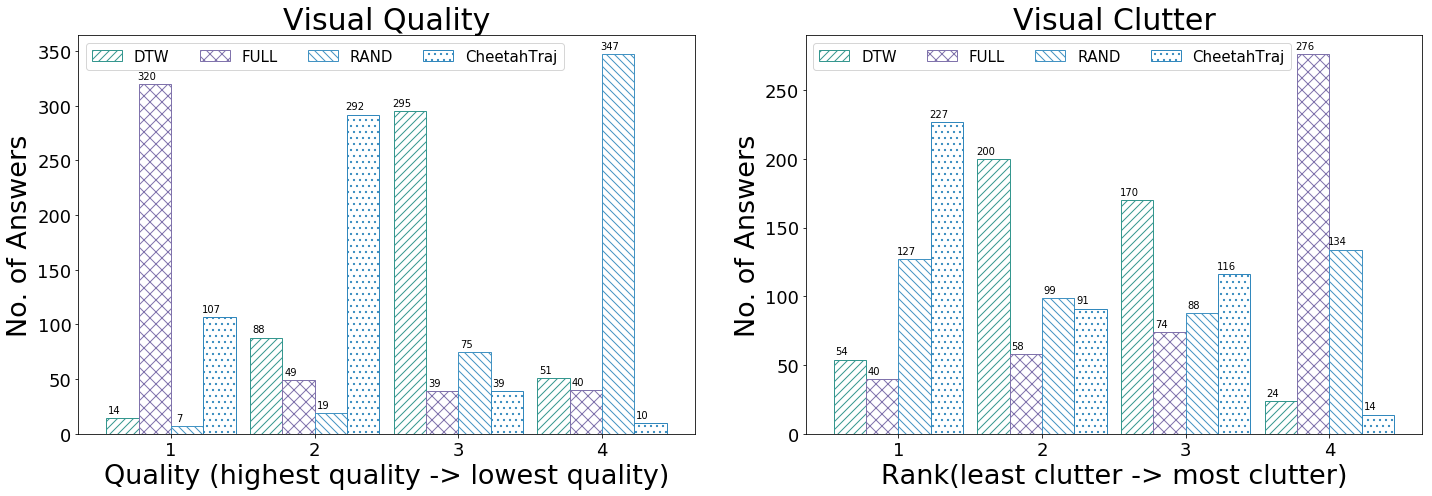
\includegraphics[width=0.6\textwidth]{pictures/user_study/rank.png}
	%\vspace{-3mm}
	\caption{User study, rank distribution.}
	\label{fig:rank}
	%\vspace{-2mm}
\end{figure*}

The left plot of Figure~\ref{fig:rank} reports the quality ranking of 4 methods in T1. The results show that $\full$ ranks the 1st in most cases while $\avats$ usually ranks 1st or 2nd. In contrast, $\mathsf{DTW}$ and $\rand$ rank 3rd and 4th in most cases. This suggests that $\avats$ outperforms $\mathsf{DTW}$ and $\rand$ in visual quality. We also found that $\avats$ ranks 1st mainly for large-scale regions in which there are many trajectories.         

 
%Figure~\ref{fig:rank} left shows the ranking among different methods with x-axis indicating the ranking from the highest quality to the lowest quality and y-axis indicating the selecting number for the specific method and ranking. The visualization of $\full$ has the highest visual quality since it has no information loss according the quality definition. The selection of $\avats$ is mostly concentrated at the first and second, which is closely behind the $\full$. The selections of $\baseline$ and $\rand$ are contracted at the third and fourth respectively, which is confirmed both of these two methods performs worse than $\full$ and $\qtavats$ in guarantee the visual quality.

The right plot of Figure~\ref{fig:rank} reports the anti-visual clutter ranking in T2. The results show that $\full$ has the most severe visual clutter, ranking 4th in most cases. $\rand$ and $\mathsf{DTW}$ reduce visual clutter via sampling, and thus usually rank 2nd and 3rd. $\avats$ is the most successful in reducing visual clutter, ranking 1st in 155 out of the xxx cases.       

%Figure~\ref{fig:rank} right reports the ranking among different methods with x-axis indicating the ranking from the least clutter to the most clutter and y-axis indicating the total selecting number for the specific method and ranking. We observe that the $\qtavats$ is ranked at the first 155 times which is significantly more than the other methods. The number it ranks at the second, third and last are 68, 96 and 14. There is no doubt that the visualization of $full$ suffers the most sever visual clutter problem because 210 of 333 total answers rank $full$ at the fourth, while other methods can be used to help to reduce the visual clutter.

We report the frequency each method is selected as acceptable and why a method is not selected for T3 using bar chart in Figure~\ref{fig:accept_rate}. Each column corresponds to a method and from left to right, the lengths of the bars means ``favorable'', ``not favorable due to visual clutter'', ``not favorable due to poor visual quality'' and ``not favorable for other reasons''. The results show that $\avats$ is acceptable in 85\% of the cases, and the other methods have significantly lower acceptance rate than $\avats$.      




\begin{figure}[t]
	\centering
	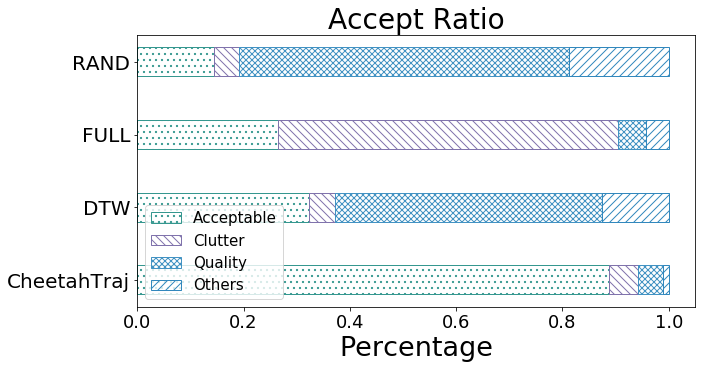
\includegraphics[width=0.35\textwidth]{pictures/user_study/accept_rate.png}
	%\vspace{-5mm}
	\caption{User study, accept rate.}
	\label{fig:accept_rate}
	%\vspace{-8mm}
\end{figure}






